% --------------------------------------------------------------
% This is all preamble stuff that you don't have to worry about.
% Head down to where it says "Start here"
% --------------------------------------------------------------
 
\documentclass[12pt]{article}

\usepackage[margin=1in]{geometry} 
\usepackage{amsmath,amsthm,amssymb,listings,xcolor,graphicx, subfig, subcaption, enumerate,framed}
 
\newenvironment{solution}{\begin{proof}[Solution]}{\end{proof}}

\definecolor{codegreen}{rgb}{0,0.6,0}
\definecolor{codegray}{rgb}{0.5,0.5,0.5}
\definecolor{codepurple}{rgb}{0.58,0,0.82}
\definecolor{backcolour}{rgb}{0.97,0.97,0.97}
\lstdefinestyle{pystyle}{
    backgroundcolor=\color{backcolour},   
    commentstyle=\color{codegreen},
    keywordstyle=\color{magenta},
    numberstyle=\tiny\color{codegray},
    stringstyle=\color{codepurple},
    basicstyle=\ttfamily\small,
    breakatwhitespace=false,         
    breaklines=true,                 
    captionpos=b,                    
    keepspaces=true,                 
    numbers=left,                    
    numbersep=5pt,                  
    showspaces=false,                
    showstringspaces=false,
    showtabs=false,                  
    tabsize=2
}
\lstset{style=pystyle}

\graphicspath{{./figures}}
 
\begin{document}
 
\title{Homework 3: Linear Approximations and Orthobases}
\author{Matthew Luyten\\ %replace with your name
ECE6250}

\maketitle

\begin{enumerate}
\item[Problem 3.1] Summary and Context of Linear Approximations and Orthobases

This week we finally got to dig into the meat of "Advanced DSP". After spending a few weeks developing a common 
language of linear algebra, we began this week talking about linear approximations in Hilbert Spaces. This is a
critical tool that allows us to perform approximations of signals like we do with a fourier series, except
we can use any basis. This significantly broadens the way we can represent and decompose signals. Also,
the fact that these opperations are all performed in linear algebra make these tools easy to use on a computer.

The other important topic we covered this week is orthobases, which make linear approximations much easier. 
These bases allow us to project a vector into their span. This makes our life much easier because we don't
have to compute a gram matrix to perform our projection.


\newpage

\item[Problem 3.2] Analog Filter Response

\begin{figure}[h]
    \caption{$N=2$}
    \centering
    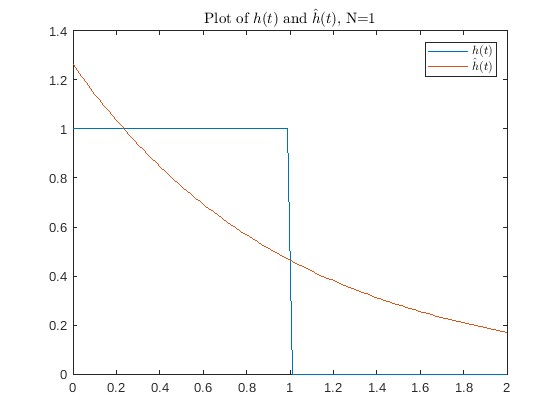
\includegraphics[scale=0.5]{3-2_a.jpg}
\end{figure}

\begin{framed}
For $N=2$, $\alpha=\begin{bmatrix}
    1.4715 \\ -0.4146
\end{bmatrix}$
\end{framed}

\begin{figure}[h]
    \caption{$N=5$}
    \centering
    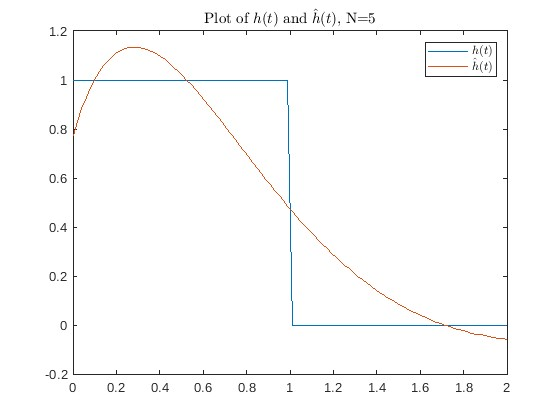
\includegraphics[scale=0.4]{3-2_b.jpg}
\end{figure}

\begin{framed}
For $N=5$, $\alpha=\begin{bmatrix}
    0.7737 \\ 3.7721 \\ -4.6012 \\ 1.4831 \\ -0.1382
\end{bmatrix}$
\end{framed}

\begin{figure}[h]
    \caption{$N=10$}
    \centering
    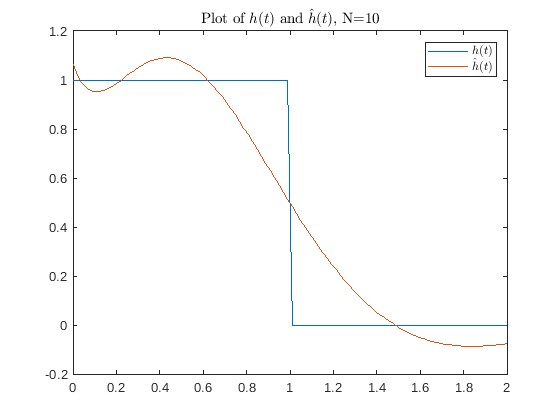
\includegraphics[scale=0.4]{3-2_c.jpg}
\end{figure}

\begin{framed}
For $N=10$, $\alpha=\begin{bmatrix}
    1.0615 \\ -1.3347 \\ 14.8125 \\-26.4481 \\ 18.8592 \\ -6.8028 \\ 1.3448 \\ -0.1465 \\ 0.0082 \\ -0.0002
\end{bmatrix}$
\end{framed}
\newpage

Code used to solve problem 3.2:

\begin{lstlisting}[language=matlab]
N=2;

% Init empty Gram and b matrices
G = zeros(N,N);
b = zeros(N,1);

% Iterate over grammian and b and fill in inner products
for r = 1:N
    for c = 1:N
        % Calc <v_c,v_r>
        f = @(t) t.^(r-1).*t.^(c-1).*exp(-2.*t);
        G(r, c) = integral(f, 0, Inf);
    end
    % Calc <x,v_r>
    f = @(t) t.^(r-1).*exp(-t);
    b(r,1) = integral(f, 0, 1);
end

% Calculate coefficients a = G^(-1)b
a = G\b;

% Plot x and x_hat (our approximation)
t = linspace(0,2);
x = t <= 1;
x_hat = zeros(1, 100);

for n = 1:N
    x_hat = x_hat + a(n).*t.^(n-1).*exp(-t);
end
plot(t, x); hold on;
plot(t, x_hat); hold off;
title(['Plot of $$h(t)$$ and $$\hat{h}(t)$$, N=', num2str(N)], 'Interpreter', 'Latex');
legend('$$h(t)$$', '$$\hat{h}(t)$$', 'Interpreter', 'Latex');
\end{lstlisting}
\newpage

\item[Problem 3.3] Norms and the Unit Ball

\begin{figure}[h]
    \caption{Unit Ball for $\|x,x\|_A$}
    \centering
    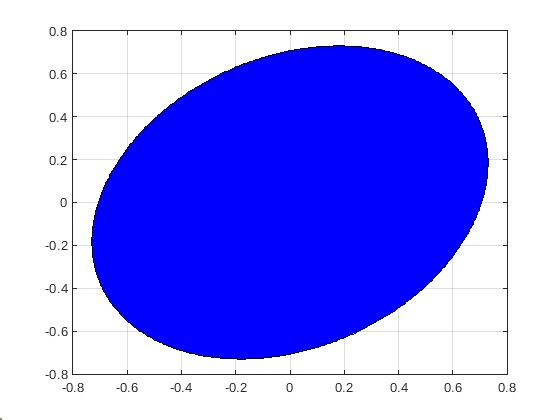
\includegraphics[scale=0.5]{3-3.jpg}
\end{figure}

Code used to solve problem 3.3:

\begin{lstlisting}[language=matlab]
% Plotting a unit ball (from lecture video)

omega = -pi:0.01:pi;
w0 = cos(omega);
w1 = sin(omega);

A = [2.0 -0.5; -0.5 2.0];
[v, lambda] = eig(A);
c = v(:,1)*w0/sqrt(lambda(1,1))+v(:,2)*w1/sqrt(lambda(2,2));
plot(c(1,:), c(2,:), 'r');
hold on; grid on;
fill(c(1,:), c(2,:), 'b')
\end{lstlisting}
\newpage

\item[Problem 3.4] Numerical Approximation with Classic Bell Curve

\begin{enumerate}
\item[] Part A

\begin{figure}[h]
    \subfloat[$\phi_k(t)$, $N=10$]{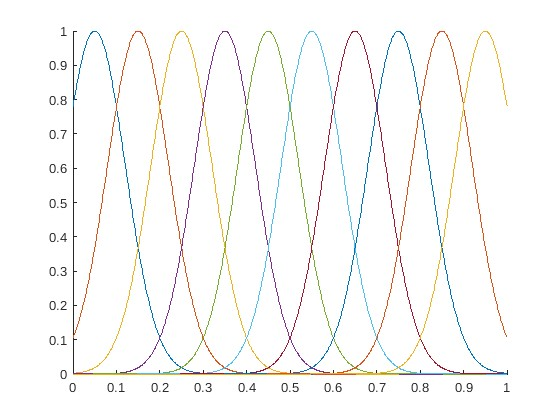
\includegraphics[width=3.2in]{3-4_a10.jpg}}
    \subfloat[$\phi_k(t)$, $N=25$]{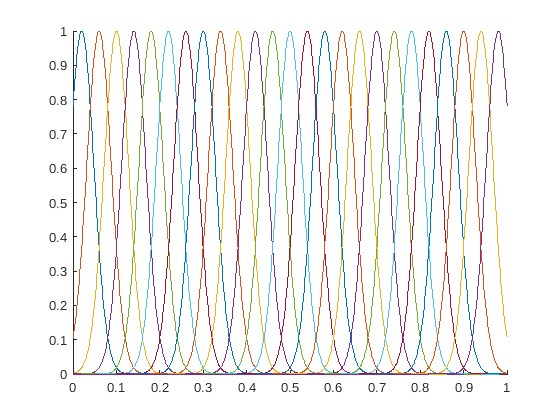
\includegraphics[width=3.2in]{3-4_a25.jpg}}
\end{figure}

\item[] Part B

\begin{figure}[h]
    \caption{$y(t)$, $N=4$, $\alpha=\begin{bmatrix} 1 & -1 & 1 & -1\end{bmatrix}^T$}
    \centering
    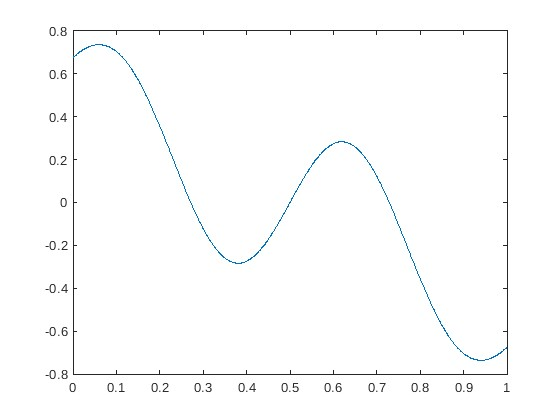
\includegraphics[scale=0.5]{3-4_b.jpg}
\end{figure}

\pagebreak

\item[] Part C

\begin{figure}[h]
    \subfloat[$N=5$]{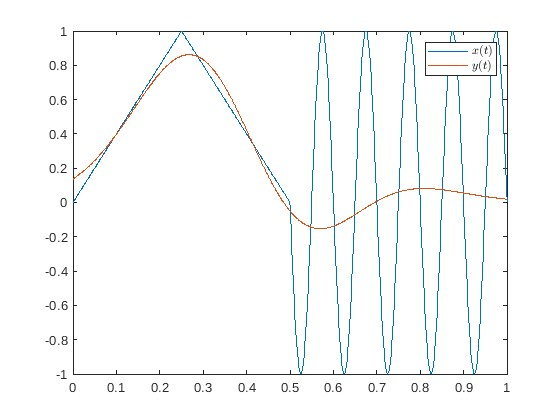
\includegraphics[width=3.2in]{3-4_c5.jpg}}
    \subfloat[$N=10$]{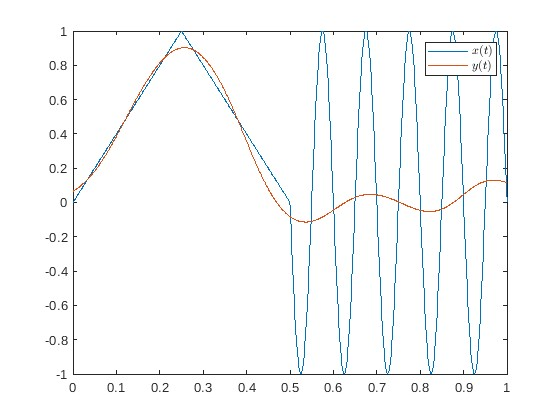
\includegraphics[width=3.2in]{3-4_c10.jpg}} \\
    \subfloat[$N=20$]{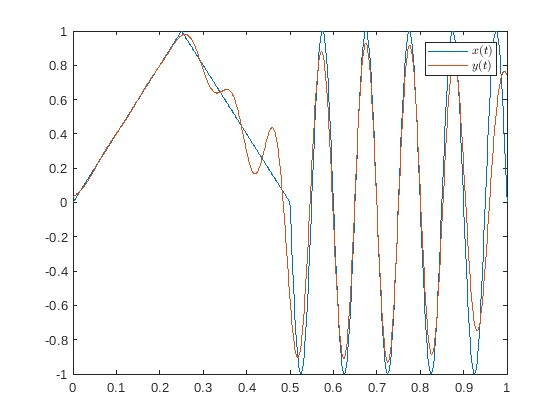
\includegraphics[width=3.2in]{3-4_c20.jpg}}
    \subfloat[$N=50$]{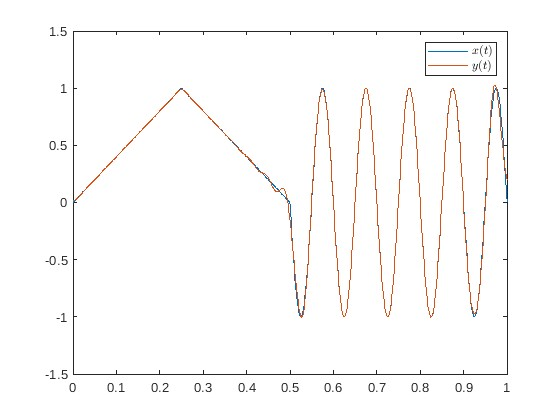
\includegraphics[width=3.2in]{3-4_c50.jpg}}
\end{figure}

\pagebreak

Code used to solve problem 3.4:

\begin{lstlisting}[language=matlab]
N=50;

% Define function and basis function
x = @(z) (z<1/4).*(4*z) + (z>=1/4).*(z<1/2).*(-4*z+2) - (z>=1/2).*sin(20*pi*z);
phi = @(z) exp(-z.^2);

% Init empty Gram and b matrices
G = zeros(N,N);
b = zeros(N,1);

% Iterate over grammian and b and fill in inner products
for r = 1:N
    for c = 1:N
        % Calc <v_c,v_r>
        f = @(t) phi(N*t - c + 1/2).*phi(N*t - r + 1/2);
        G(r, c) = integral(f, 0, Inf);
    end
    % Calc <x,v_r>
    f = @(t) x(t).*phi(N*t - r + 1/2);
    b(r,1) = integral(f, 0, 1);
end

% Calculate coefficients a = G^(-1)b
a = G\b;

% Create t, x(t), and y(t) and 
t = linspace(0,1,1000);
x = x(t);
y = zeros(size(t));

for jj = 1:N
    y = y + a(jj)*phi(N*t - jj + 1/2);
end

% Plot 'em
figure(1);
plot(t,x); hold on
plot(t,y); hold off
legend('$$x(t)$$', '$$y(t)$$', 'Interpreter', 'Latex');
\end{lstlisting}

\end{enumerate}

\end{enumerate}


\end{document}
